%% AIQxQIA 2026 -- CEUR-WS submission.
%% Single-blind: author names ARE included, so the `singleblind' class option
%% (which anonymises) is deliberately NOT passed. One column is the ceurart default
%% and the CEUR house layout.
\documentclass{ceurart}

%% Latin Modern: scalable Type1, so microtype's font expansion works. Without it,
%% T1 Computer Modern falls back to bitmaps here (no cm-super installed) and pdfTeX
%% aborts with "auto expansion is only possible with scalable fonts".
\usepackage{lmodern}
\usepackage{amsmath,amssymb,amsthm}
\usepackage{booktabs}
\usepackage{graphicx}
\usepackage{todonotes}
\setuptodonotes{inline,color=yellow!40}

% Generated by code/experiments/collect_numbers.py -- do not edit by hand.
% Rerun: uv run python -m experiments.collect_numbers
\providecommand{\EOneDataset}{}\renewcommand{\EOneDataset}{wordnet}
\providecommand{\EOneLeaves}{}\renewcommand{\EOneLeaves}{256}
\providecommand{\EOneHeight}{}\renewcommand{\EOneHeight}{8}
\providecommand{\EOneSourceNodes}{}\renewcommand{\EOneSourceNodes}{74\,374}
\providecommand{\EOneSourceHeight}{}\renewcommand{\EOneSourceHeight}{19}
\providecommand{\EOneLevels}{}\renewcommand{\EOneLevels}{9}
\providecommand{\PathStateNodes}{}\renewcommand{\PathStateNodes}{1\,028}
\providecommand{\PathStateQubits}{}\renewcommand{\PathStateQubits}{11}
\providecommand{\PathResidual}{}\renewcommand{\PathResidual}{4.44 \times 10^{-16}}
\providecommand{\PathViolations}{}\renewcommand{\PathViolations}{0}
\providecommand{\PathLevelConstancy}{}\renewcommand{\PathLevelConstancy}{4.44 \times 10^{-16}}
\providecommand{\PathResolution}{}\renewcommand{\PathResolution}{9}
\providecommand{\BasisViolations}{}\renewcommand{\BasisViolations}{0}
\providecommand{\BasisResolution}{}\renewcommand{\BasisResolution}{2}
\providecommand{\AngleViolationRate}{}\renewcommand{\AngleViolationRate}{0.322}
\providecommand{\AngleLevelConstancy}{}\renewcommand{\AngleLevelConstancy}{0.978}
\providecommand{\ZZViolationRate}{}\renewcommand{\ZZViolationRate}{0.328}
\providecommand{\ZZLevelConstancy}{}\renewcommand{\ZZLevelConstancy}{0.48}
\providecommand{\RandProdViolationRate}{}\renewcommand{\RandProdViolationRate}{0.329}
\providecommand{\RandProdLevelConstancy}{}\renewcommand{\RandProdLevelConstancy}{0.991}
\providecommand{\RBFViolations}{}\renewcommand{\RBFViolations}{5\,527\,040}
\providecommand{\NCBIRadix}{}\renewcommand{\NCBIRadix}{38}
\providecommand{\ETwoLeaves}{}\renewcommand{\ETwoLeaves}{255}
\providecommand{\ETwoClasses}{}\renewcommand{\ETwoClasses}{10}
\providecommand{\ETwoPathAccuracy}{}\renewcommand{\ETwoPathAccuracy}{0.792}
\providecommand{\ETwoPathAccuracyStd}{}\renewcommand{\ETwoPathAccuracyStd}{0.0157}
\providecommand{\ETwoPathRho}{}\renewcommand{\ETwoPathRho}{1}
\providecommand{\ETwoBestBaseline}{}\renewcommand{\ETwoBestBaseline}{random product}
\providecommand{\ETwoBestBaselineAccuracy}{}\renewcommand{\ETwoBestBaselineAccuracy}{0.839}
\providecommand{\ETwoBestBaselineRho}{}\renewcommand{\ETwoBestBaselineRho}{0.368}
\providecommand{\EThreeConfigs}{}\renewcommand{\EThreeConfigs}{56}
\providecommand{\EThreeWorstResidual}{}\renewcommand{\EThreeWorstResidual}{2.22 \times 10^{-16}}
\providecommand{\EThreeMaxViolations}{}\renewcommand{\EThreeMaxViolations}{0}
\providecommand{\QubitBoundPTwo}{}\renewcommand{\QubitBoundPTwo}{4.43}
\providecommand{\QubitBoundPThree}{}\renewcommand{\QubitBoundPThree}{7.51}
\providecommand{\QubitBoundPFive}{}\renewcommand{\QubitBoundPFive}{11.3}
\providecommand{\EFourConfigs}{}\renewcommand{\EFourConfigs}{120}
\providecommand{\EFourExactAlignment}{}\renewcommand{\EFourExactAlignment}{0.421}
\providecommand{\EFourBestAlignment}{}\renewcommand{\EFourBestAlignment}{0.426}
\providecommand{\EFourBestDistortion}{}\renewcommand{\EFourBestDistortion}{0.0464}
\providecommand{\EFourAlignmentGain}{}\renewcommand{\EFourAlignmentGain}{0.00459}
\providecommand{\ShotBudget}{}\renewcommand{\ShotBudget}{100\,000}
\providecommand{\ShotTargetExcess}{}\renewcommand{\ShotTargetExcess}{0.01}
\providecommand{\TieFraction}{}\renewcommand{\TieFraction}{0.667}
\providecommand{\ENoiseRepeats}{}\renewcommand{\ENoiseRepeats}{10}
\providecommand{\ExcessAtLowShots}{}\renewcommand{\ExcessAtLowShots}{0.134}
\providecommand{\ExcessAtLowShotsCount}{}\renewcommand{\ExcessAtLowShotsCount}{100}
\providecommand{\ExcessAtHighShots}{}\renewcommand{\ExcessAtHighShots}{0.00165}
\providecommand{\ExcessAtHighShotsCount}{}\renewcommand{\ExcessAtHighShotsCount}{1\,000\,000}


%% ---------------------------------------------------------------- notation macros
\newcommand{\Zp}{\mathbb{Z}_p}
\newcommand{\Zpn}{\mathbb{Z}/p^{n}}
\newcommand{\C}{\mathbb{C}}
\newcommand{\R}{\mathbb{R}}
\newcommand{\Nat}{\mathbb{N}}
\newcommand{\vp}{v_p}
\newcommand{\lcadepth}{\lambda}
\newcommand{\pathstate}[1]{\Phi_f(#1)}
\newcommand{\fid}[2]{\lvert\langle #1 \mid #2 \rangle\rvert^{2}}
\newcommand{\ket}[1]{\lvert #1 \rangle}
\newcommand{\bra}[1]{\langle #1 \rvert}
\newcommand{\braket}[2]{\langle #1 \mid #2 \rangle}
\newcommand{\abs}[1]{\lvert #1 \rvert}
\newcommand{\norm}[1]{\lVert #1 \rVert}
\DeclareMathOperator{\anc}{anc}
\DeclareMathOperator{\rank}{rank}
\DeclareMathOperator*{\Tr}{tr}

\theoremstyle{plain}
\newtheorem{theorem}{Theorem}
\newtheorem{proposition}[theorem]{Proposition}
\newtheorem{corollary}[theorem]{Corollary}
\newtheorem{lemma}[theorem]{Lemma}
\theoremstyle{definition}
\newtheorem{definition}[theorem]{Definition}
\newtheorem{remark}[theorem]{Remark}
\newtheorem{example}[theorem]{Example}

\begin{document}

\copyrightyear{2026}
\copyrightclause{Copyright for this paper by its author.
  Use permitted under Creative Commons License Attribution 4.0
  International (CC BY 4.0).}

\conference{AIQxQIA 2026: International Workshop on AI for Quantum and Quantum for AI,
  2026}

\title{Ultrametric Quantum Kernels: Exact $p$-adic Feature Maps for Hierarchical Data}

\author[1]{TODO-AUTHOR}[
  email=todo@example.org,
]
\address[1]{TODO-AFFILIATION}

\todo{BLOCKER: author name, affiliation, ORCID and email are placeholders. The paper
must not be uploaded while the string TODO-AUTHOR appears anywhere in the source.}

\begin{abstract}
  \todo{Written last, once every number is final.}
\end{abstract}

\begin{keywords}
  quantum machine learning \sep
  quantum kernels \sep
  ultrametric spaces \sep
  $p$-adic numbers \sep
  hierarchical representation learning
\end{keywords}

\maketitle

%% 01-introduction
\section{Introduction}
\label{sec:introduction}

\todo{Draft pending.}

%% 02-preliminaries
\section{Preliminaries}
\label{sec:preliminaries}

\todo{Draft pending.}

%% 03-problem
\section{Ultrametric Quantum Kernels}
\label{sec:problem}

\todo{Draft pending.}

%% 04-theorem-a
\section{A No-Go Theorem for Product Encodings}
\label{sec:theorem-a}

\begin{theorem}[Product no-go]
  \label{thm:product-nogo}
  Let $\Phi$ be a block-product feature map on $\Zpn$ (\Cref{def:block-product-map})
  whose fidelity kernel is ultrametric with profile $f$, and set
  $v^{*} = \min\{\, v : f(v) > 0 \,\}$. Let $B^{*}$ be the block containing level
  $v^{*}+1$. Then for every block $B$ all of whose levels exceed $\max B^{*}$, and all
  digit tuples $a, b$,
  \begin{equation}
    \label{eq:trivial-block}
    \abs{\braket{\psi_B(a)}{\psi_B(b)}} = 1 .
  \end{equation}
  Consequently $f$ takes at most the three values $\{0, f(v^{*}), 1\}$, and $\Phi$
  resolves the tree only to depth $\max B^{*}$. In particular, for a product map with
  $n \ge 2$, no strictly monotone profile is realisable.
\end{theorem}

\begin{proof}
  The argument uses exactly one property of the encoding: fidelity is multiplicative
  across tensor factors, \cref{eq:multiplicative}. We give it for $v^{*} = 0$; the
  general case shifts every index by $v^{*}$, since all pairs meeting above depth
  $v^{*}$ have kernel value $0$ and impose no constraint.

  Let $B$ be a block whose levels all exceed $\max B^{*}$, and fix digit tuples
  $a \ne b$ for it. Choose leaves $x, y$ that differ in level $1$ and agree at every
  other level, with $x_B = a$. Then $\lcadepth(x,y) = 0$, and since every factor other
  than $B^{*}$ contributes $g(x, x) = 1$,
  \begin{equation}
    \label{eq:base-value}
    f(0) = K(x, y) = \fid{\psi_{B^{*}}(x_{B^{*}})}{\psi_{B^{*}}(y_{B^{*}})} .
  \end{equation}

  Now let $y'$ agree with $y$ everywhere except on $B$, where $y'_B = b$. Because $x$
  and $y'$ still differ at level $1$, and $B$ does not contain level $1$, we still have
  $\lcadepth(x, y') = 0$ and therefore $K(x, y') = f(0)$. But multiplicativity gives
  \begin{equation*}
    K(x, y')
    = \fid{\psi_{B^{*}}(x_{B^{*}})}{\psi_{B^{*}}(y_{B^{*}})} \cdot
      \fid{\psi_{B}(a)}{\psi_{B}(b)}
    = f(0) \cdot \fid{\psi_B(a)}{\psi_B(b)} .
  \end{equation*}
  Since $f(0) > 0$ by the choice $v^{*} = 0$, this forces
  $\fid{\psi_B(a)}{\psi_B(b)} = 1$, which is \cref{eq:trivial-block}: the states of
  block $B$ coincide up to a global phase, and $B$ carries no information about the
  data.

  Every block beyond $B^{*}$ being trivial, $K$ depends only on the digits in blocks up
  to $B^{*}$. Two leaves agreeing down to depth $\max B^{*}$ therefore have
  $K(x,y) = 1$, so $f(v) = 1$ for all $v > \max B^{*}$ --- the tree is resolved no
  deeper. Level constancy forces the common value $f(0)$ on all pairs meeting at the
  root, so together with the vanishing values below $v^{*}$ the profile takes at most
  the three values $\{0, f(v^{*}), 1\}$. For a product map every block is a single
  level, $\max B^{*} = v^{*}+1$, and a strictly monotone profile would need $n+1$
  distinct values, which exceeds three whenever $n \ge 2$.
\end{proof}

The proof turns on multiplicativity alone. It is therefore indifferent to the local
dimensions $d_i$, to whether the local states are real or complex, and to how they were
chosen --- which is what makes it a statement about a class of encodings rather than
about particular instances.

\begin{corollary}
  \label{cor:standard-encodings}
  On $\Zpn$ with $n \ge 2$, none of the following induces a strictly monotone
  ultrametric kernel: angle encoding with one qubit per digit; computational-basis
  encoding; and any first-order Pauli-$Z$ feature map, whose phase is a sum of
  single-digit terms and which is therefore a product map.
\end{corollary}

Basis encoding is the extreme case and deserves a sentence, because it is the one that
can be mistaken for a success. It attains $v^{*} = n$: its kernel is the identity, its
induced distance is the discrete metric, and it satisfies \cref{eq:strong-triangle}
with zero violations while resolving nothing. It is a corner of
\Cref{thm:product-nogo}, not a counterexample to it, and it is the reason
\Cref{subsec:diagnostics} insists on reporting resolution depth alongside violations.

\begin{remark}[What this theorem does not cover]
  \label{rem:not-covered}
  A ZZ or IQP feature map applies all-pairs couplings between qubits, so its state does
  not factorise across digits and \cref{eq:multiplicative} fails. \Cref{thm:product-nogo}
  says nothing about it. We do not patch the gap by weakening the claim; we close it in
  \Cref{sec:theorem-b} with an argument that ignores the structure of the encoding
  entirely.
\end{remark}

\paragraph{Numerical verification.}
Randomly drawn product maps are never level-constant for
$(p, n) \in \{(2,3), (3,2), (2,4), (5,2)\}$ across five seeds
(\texttt{test\_theorem\_a\_random\_product\_maps\_are\_never\_strictly\_monotone}). A
product map built to satisfy the conclusion --- one non-trivial level, the rest trivial
--- yields exactly two distinct kernel values, as predicted
(\texttt{test\_theorem\_a\_ultrametric\_product\_map\_resolves\_only\_one\_level}), and
switching on a second non-trivial level destroys level constancy, which is the
contradiction the proof derives
(\texttt{test\_theorem\_a\_a\_nontrivial\_deep\_factor\_destroys\_ultrametricity}).

%% 05-theorem-b
\section{A Dimension Lower Bound for Arbitrary Encodings}
\label{sec:theorem-b}

\todo{Draft pending.}

%% 06-theorem-c
\section{Exact Realisation by Path States}
\label{sec:theorem-c}

The two obstructions leave a gap: strictly monotone ultrametric kernels need many
dimensions and cannot be factorised across digits. The construction in this section
fills the gap exactly, and turns out to characterise the whole family.

\begin{theorem}[Path states]
  \label{thm:path-states}
  Let $T$ be a finite rooted tree on node set $V$ with all leaves at depth $n$. For
  every strictly increasing $f : \{0, \dots, n\} \to (0, 1]$ with $f(n) = 1$, set
  \begin{equation}
    \label{eq:amplitudes}
    a_i^{2} = \sqrt{f(i)} - \sqrt{f(i-1)} \quad (0 \le i \le n), \qquad
    \sqrt{f(-1)} := 0,
  \end{equation}
  and define the \emph{path state}
  \begin{equation}
    \label{eq:path-state}
    \pathstate{x} \;=\; \sum_{i=0}^{n} a_i \ket{\anc_i(x)} \;\in\; \C^{V} .
  \end{equation}
  Then $\pathstate{x}$ is a unit vector and, for all leaves $x, y$,
  \begin{equation}
    \label{eq:exactness}
    \fid{\pathstate{x}}{\pathstate{y}} = f\bigl(\lcadepth(x,y)\bigr) \qquad
    \text{exactly.}
  \end{equation}
  Conversely, every kernel that is ultrametric with a strictly monotone profile arises
  this way, and $\Phi_f$ is the unique realisation up to a global isometry and a phase
  on each point \emph{among realisations whose pairwise overlaps are real and
  non-negative}. Dropping that restriction, uniqueness fails
  (\Cref{rem:uniqueness}).
\end{theorem}

\begin{proof}
  Strict monotonicity makes each $a_i^{2}$ in \cref{eq:amplitudes} positive, so the
  $a_i$ are well defined and real. The sum telescopes,
  $\sum_{i=0}^{n} a_i^{2} = \sqrt{f(n)} = 1$, so $\pathstate{x}$ is a unit vector.

  For the overlap, the key structural fact is that two leaves share precisely their
  ancestors down to the depth at which they meet, and no deeper: $\anc_i(x) = \anc_i(y)$
  if and only if $i \le \lcadepth(x,y)$. The basis vectors $\ket{u}$ for $u \in V$ being
  orthonormal,
  \begin{equation}
    \label{eq:overlap}
    \braket{\pathstate{x}}{\pathstate{y}}
    = \sum_{i=0}^{n} a_i^{2} \,\mathbf{1}\bigl[\anc_i(x) = \anc_i(y)\bigr]
    = \sum_{i \le \lcadepth(x,y)} a_i^{2}
    = \sqrt{f\bigl(\lcadepth(x,y)\bigr)} ,
  \end{equation}
  again by telescoping. Squaring the modulus gives \cref{eq:exactness}.

  Two remarks on \cref{eq:overlap}. The cross terms vanish because $\anc_i(x)$ and
  $\anc_j(y)$ sit at different depths when $i \ne j$, so they are distinct nodes and
  hence orthogonal basis vectors. And $a_i^{2} = \sqrt{f(i)} - \sqrt{f(i-1)}$ is forced
  by \cref{eq:overlap} read at successive levels, so $f$ determines the amplitudes.

  For the converse, let $\Psi$ be a realisation whose Gram matrix $G^{\Psi}$ has real
  non-negative entries. Then $G^{\Psi}_{xy} = \sqrt{f(\lcadepth(x,y))}$ exactly, which
  by \cref{eq:overlap} is the Gram matrix of $\Phi_f$. Two families of vectors with
  equal Gram matrices are related by an isometry of their spans, which is the standard
  argument; composing with per-point phases covers the residual freedom that leaves
  $\abs{\cdot}$ unchanged.
\end{proof}

\begin{remark}[How far uniqueness actually goes]
  \label{rem:uniqueness}
  Two weakenings are needed, and the second is not cosmetic.

  First, the converse cannot say ``unique up to relabelling of $V$''. Rotating every
  $\pathstate{x}$ by a fixed unitary, or multiplying each by its own phase, leaves the
  fidelity kernel unchanged while destroying the reading of the basis as tree nodes
  (\texttt{test\_theorem\_c\_uniqueness\_up\_to\_isometry\_and\_phase}). The
  node-labelled form \cref{eq:path-state} is the canonical representative of its
  isometry class, not the only member.

  Second, and less obviously, the positivity hypothesis cannot be dropped. A fidelity
  kernel fixes only the \emph{moduli} $\abs{G_{xy}}$, and these do not determine $G$ up
  to phases: the Bargmann invariants $G_{xy}G_{yz}G_{zx}$ are invariant under
  $\Psi(x) \mapsto e^{i\vartheta_x} U \Psi(x)$ yet are not functions of the moduli.
  Concretely, take $n = 1$, $p = 3$, $f(0) = t = 1/4$ and
  \begin{equation*}
    G^{\Psi} =
    \begin{pmatrix}
      1 & \sqrt{t} & i\sqrt{t} \\
      \sqrt{t} & 1 & \sqrt{t} \\
      -i\sqrt{t} & \sqrt{t} & 1
    \end{pmatrix},
  \end{equation*}
  which is positive semi-definite with spectrum $\{0.134, 1, 1.866\}$ and realises the
  same kernel as $\Phi_f$. Its Bargmann invariant is $-\tfrac{1}{8}i$ against
  $+\tfrac{1}{8}$ for the path state, so no isometry and no choice of phases carries one
  to the other. The correspondence $f \leftrightarrow \Phi_f$ is therefore a bijection
  onto strictly monotone ultrametric kernels only after restricting to realisations with
  non-negative overlaps
  (\texttt{test\_theorem\_c\_converse\_needs\_non\_negative\_overlaps}).
\end{remark}

\begin{remark}[Positive semi-definiteness for free]
  \label{rem:psd}
  Let $A$ be the leaf-by-node incidence matrix with $A_{xu} = a_{\mathrm{depth}(u)}$ if
  $u$ is an ancestor of $x$ and $0$ otherwise. Then \cref{eq:overlap} says
  $\sqrt{K} = A A^{\!\top}$ entrywise, so $K = (A A^{\!\top})^{\circ 2}$ is a Schur
  square of a positive semi-definite matrix and hence positive semi-definite. This
  re-derives, in one line, the classical fact that monotone ultrametric kernels are
  positive semi-definite.
\end{remark}

\subsection{Resources}
\label{subsec:resources}

The path state lives in $\C^{V}$, so it needs $\lceil \log_2 \abs{V} \rceil$ qubits.
Critically, it has only $n+1$ non-zero amplitudes out of $\abs{V}$, so it is a sparse
state. In a level-indexed layout, where the register splits into a depth counter and a
within-level index, preparation is a cascade of $n$ controlled rotations --- one per
level, each splitting the remaining amplitude between ``stop here'' and ``descend'' ---
followed, at each level, by writing the within-level index of $\anc_i(x)$ conditioned on
the depth register. Counting both parts gives $O(n \log \abs{V})$ elementary gates. We
quote that figure throughout; the $O(n)$ rotations alone are not the whole cost.

\begin{table}
  \centering
  \caption{Resources for the path-state encoding, and the \Cref{thm:dimension-bound}
    bound it must respect. Dataset rows use the depth-8 truncation of
    \Cref{sec:experiments}; the WordNet row is the full hierarchy before truncation.}
  \label{tab:resources}
  \begin{tabular}{lrrrr}
    \toprule
    & nodes $\abs{V}$ & qubits & non-zero amplitudes & preparation gates \\
    \midrule
    general tree & $\abs{V}$ & $\lceil \log_2 \abs{V} \rceil$ & $n+1$
      & $O(n \log \abs{V})$ \\
    $\Zpn$ & $\frac{p^{n+1}-1}{p-1}$ & $\approx n \log_2 p$ & $n+1$ & $O(n^{2}\log p)$ \\
    WordNet (full) & $\EOneSourceNodes$ & $17$ & $\EOneSourceHeight + 1$ & --- \\
    WordNet (truncated) & $\PathStateNodes$ & $\PathStateQubits$ & $\EOneHeight + 1$
      & --- \\
    \bottomrule
  \end{tabular}
\end{table}

\Cref{tab:resources} collects the counts. The headline is that the full WordNet noun
hierarchy --- $\EOneSourceNodes$ nodes --- fits in $17$ qubits, with $\EOneSourceHeight
+ 1$ non-zero amplitudes.

\paragraph{Optimality.}
Comparing with \Cref{cor:no-n-qubit}: on $\Zpn$ the construction uses
$\log_2 \abs{V} = n \log_2 p + \log_2 \frac{p}{p-1} + o(1)$ qubits, while the bound
demands at least $n \log_2 p - \log_2 S(p,s)$. The two differ by an additive constant
independent of $n$, so the path-state encoding is optimal up to $O(1)$ qubits. We
resist the stronger phrasing: it is not exactly optimal, and the gap is a genuine, if
small, one.

\subsection{The $p$-adic specialisation}
\label{subsec:padic-specialisation}

On the regular $p$-ary tree, $\lcadepth(x,y) = \min(\vp(x-y), n)$ and the profile can
be tied directly to the $p$-adic absolute value. With $\abs{x-y}_p = p^{-\lcadepth}$ for
$x \ne y$, the geometric profile is
\begin{equation}
  \label{eq:padic-profile}
  f(\lcadepth) = p^{-(n-\lcadepth)s}
  = \Bigl( \frac{p^{-n}}{\abs{x-y}_p} \Bigr)^{\!s} ,
\end{equation}
so the kernel is a decreasing power of the $p$-adic distance, with $f(n) = 1$ filling in
the value at $x = y$ where $\abs{x-y}_p = 0$. The path state is then a level-weighted superposition over the
root-to-leaf path in the $p$-adic tree, with amplitude concentrated near the leaf for
large $s$ and spread towards the root for small $s$. This is the same object that
appears as the state space of continuous-time quantum walks on $p$-adic trees, where
the vertices are sub-balls of a $p$-adic ball
\citep{ZunigaGalindo2024QuantumWalks,ZunigaGalindo2025TwoAdic}, and it connects the
encoding to the $p$-adic quantum formalism of \citet{AnielloEtAl2023PadicQubit}.

\subsection{Arbitrary rooted trees}
\label{subsec:general-trees}

Nothing in the proof of \Cref{thm:path-states} uses regularity. The only structural
input is \cref{eq:overlap}, which needs just that ancestors nest --- true in any rooted
tree. Branching factors may vary between nodes and between levels, and shallow leaves
are handled by the unary padding of \Cref{sec:problem}, which changes no lowest common
ancestor. The construction therefore applies verbatim to WordNet, whose branching
factor ranges from $1$ to $402$, and $\Zpn$ is the homogeneous specialisation rather
than the setting
(\texttt{test\_theorem\_c\_generalises\_to\_a\_non\_homogeneous\_tree}).

\paragraph{Numerical verification.}
Across $(p,n) \in \{(2,3), (3,2), (2,4), (5,2)\}$ and both geometric and linear
profiles, the residual $\max_{x,y} \abs{K - f(\lcadepth)}$ is at most
$\EThreeWorstResidual$, and the induced distance has zero strong-triangle violations
(\texttt{test\_theorem\_c\_path\_states\_realise\_the\_profile\_exactly},
\texttt{test\_theorem\_c\_induced\_distance\_is\_exactly\_ultrametric}).

%% 07-reuploading
\section{Beyond Exactness: Re-uploading and Noise}
\label{sec:reuploading}

\todo{Draft pending.}

%% 08-experiments
\section{Experiments}
\label{sec:experiments}

All experiments are analytic or statevector simulations on CPU, using NumPy and
scikit-learn, and each completes in seconds to minutes. Seeds, resolved configurations
and library versions are recorded alongside every run. Every number quoted below is
generated from the experiment outputs rather than transcribed by hand.

\subsection{Setup}
\label{subsec:setup}

\paragraph{Datasets.}
We use WordNet nouns via NLTK, the molecular-function namespace of the Gene Ontology,
the Mammalia clade of the NCBI taxonomy, and synthetic regular $p$-ary trees for
controlled ablations. \Cref{tab:datasets} gives the shapes.

\begin{table}
  \centering
  \caption{The four hierarchies after preprocessing. Source columns describe the full
    reduced tree; the remaining columns describe the sample the kernels are evaluated
    on. Qubits is $\lceil \log_2 \abs{V} \rceil$ for the path-state encoding.}
  \label{tab:datasets}
  \small
  % Generated by code/experiments/collect_numbers.py -- do not edit.
\begin{tabular}{lrrrrrr}
\toprule
dataset & source nodes & source height & sampled leaves & nodes & radix & qubits \\
\midrule
synthetic $2$-ary & $511$ & $8$ & $256$ & $511$ & $2$ & $9$ \\
WordNet & $74\,374$ & $19$ & $256$ & $1\,028$ & $11$ & $11$ \\
Gene Ontology & $10\,041$ & $12$ & $256$ & $1\,235$ & $16$ & $11$ \\
NCBI Mammalia & $14\,722$ & $14$ & $256$ & $633$ & $38$ & $10$ \\
\bottomrule
\end{tabular}

\end{table}

\paragraph{Preprocessing, stated rather than assumed.}
Each of these sources is a directed acyclic graph in the wild, not a tree: WordNet
synsets can have several hypernyms. We reduce each to a tree by keeping, for every
node, the \emph{longest} path to the root, breaking ties by lexicographically smallest
identifier. Multiple inheritance is therefore discarded, which we record as a
limitation in \Cref{sec:limitations} rather than as a detail.

We then truncate every hierarchy at depth $\EOneHeight$. This is needed because the
$2^{\text{height}}$-dimensional product baselines are otherwise not representable:
WordNet reaches depth $\EOneSourceHeight$, so an angle or ZZ encoding would require
$2^{\EOneSourceHeight}$ amplitudes per point. Truncation also has the further benefit that
every encoding is compared on exactly the same tree. Finally we sample $\EOneLeaves$ leaves,
restrict to their ancestor closure, and pad shallow leaves to uniform depth. None of
these steps changes the lowest-common-ancestor depths among the sampled leaves below
the truncation, which is all the kernel depends on.

\paragraph{Baselines.}
Angle encoding, computational-basis encoding, a ZZ/IQP feature map with two
repetitions, a random product map, a block-product map where representable, and two
classical references: an RBF kernel on integer leaf coordinates and one on a one-hot
encoding. The geometric profile uses base $2$ throughout for the real datasets. Tying
the profile base to the branching factor instead, $\NCBIRadix$ for NCBI, pushes
$f(0)$ to around $10^{-13}$, below any resolution tolerance that a realistic shot
budget could support, so the base is treated as the free design parameter it is.

\subsection{E1: ultrametricity and resolution}
\label{subsec:e1}

\Cref{tab:e1} reports both diagnostics of \Cref{def:diagnostics} across all four
hierarchies, and \Cref{fig:e1-violations} plots them for WordNet.

\begin{table}
  \centering
  \caption{E1. Violation rate counts triples breaking \cref{eq:strong-triangle}; level
    constancy is zero exactly when the kernel is ultrametric with some profile;
    resolution is the number of distinguishable kernel values against the number of
    lowest-common-ancestor levels the sample populates. Only the path state scores well
    on both.}
  \label{tab:e1}
  \small
  % Generated by code/experiments/collect_numbers.py -- do not edit.
\begin{tabular}{llrrr}
\toprule
dataset & encoding & violation rate & level constancy & resolution \\
\midrule
synthetic $2$-ary & \textbf{path state (ours)} & $0$ & $0$ & 9 / 9 \\
 & basis & $0$ & $0$ & 2 / 9 \\
 & angle & $0.234$ & $0.496$ & 9 / 9 \\
 & ZZ / IQP & $0.275$ & $0.983$ & 9 / 9 \\
 & random product & $0.329$ & $0.927$ & 9 / 9 \\
\addlinespace
WordNet & \textbf{path state (ours)} & $0$ & $4.44 \times 10^{-16}$ & 9 / 9 \\
 & basis & $0$ & $0$ & 2 / 9 \\
 & angle & $0.322$ & $0.978$ & 9 / 9 \\
 & ZZ / IQP & $0.328$ & $0.48$ & 9 / 9 \\
 & random product & $0.329$ & $0.991$ & 9 / 9 \\
\addlinespace
Gene Ontology & \textbf{path state (ours)} & $0$ & $4.44 \times 10^{-16}$ & 9 / 9 \\
 & basis & $0$ & $0$ & 2 / 9 \\
 & angle & $0.322$ & $0.986$ & 9 / 9 \\
 & ZZ / IQP & $0.327$ & $0.748$ & 9 / 9 \\
 & random product & $0.329$ & $0.992$ & 9 / 9 \\
\addlinespace
NCBI Mammalia & \textbf{path state (ours)} & $0$ & $4.44 \times 10^{-16}$ & 9 / 9 \\
 & basis & $0$ & $0$ & 2 / 9 \\
 & angle & $0.323$ & $0.998$ & 9 / 9 \\
 & ZZ / IQP & $0.328$ & $0.605$ & 9 / 9 \\
 & random product & $0.329$ & $0.999$ & 9 / 9 \\
\addlinespace
\bottomrule
\end{tabular}

\end{table}

\begin{figure}
  \centering
  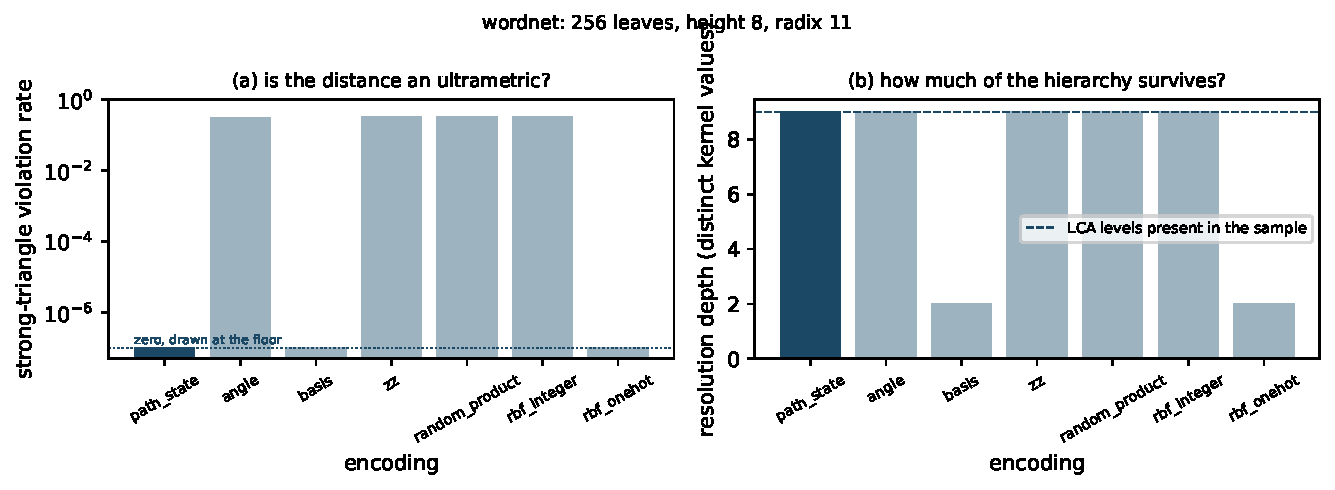
\includegraphics[width=\linewidth]{figures/e1_violations}
  \caption{E1 on WordNet. Panel~(a) asks whether the induced distance is an ultrametric
    at all; panel~(b) asks how much of the hierarchy survives. Basis encoding passes
    (a) perfectly and fails (b) completely, which is why both are reported.}
  \label{fig:e1-violations}
\end{figure}

Three readings. First, the path-state encoding attains level constancy
$\PathLevelConstancy$ and zero violations on every dataset, with full resolution: the
construction is exact on real hierarchies, not only on the regular trees of
\Cref{thm:path-states}. Second, every product and entangling baseline has a level
constancy near $1$: angle reaches $\AngleLevelConstancy$ and the random product map
$\RandProdLevelConstancy$. Their kernels are not merely imperfect ultrametrics
but are not ultrametric at all, in agreement with \Cref{thm:product-nogo,thm:dimension-bound}.

Third, and worth stating plainly because it complicates the headline: \textbf{basis
encoding also achieves zero violations}, with level constancy exactly zero. Its
resolution is $\BasisResolution$ out of $\EOneLevels$. This is the degenerate corner of
\Cref{thm:product-nogo} discussed in \Cref{sec:theorem-a}, and it is the reason we do
not claim that the path state is the unique encoding with an ultrametric kernel. The
correct claim is narrower and, we think, more useful: it is the only one that is both
ultrametric and fully resolving.

\subsection{E2: hierarchical classification}
\label{subsec:e2}

\Cref{tab:e2} reports five-fold cross-validated accuracy for predicting a leaf's
depth-$2$ ancestor, together with the Spearman correlation between the kernel's induced
distance and true tree distance. Classes with fewer than five members are dropped and
the count is reported in the run metadata; no hyperparameter was tuned.

\begin{table}
  \centering
  \caption{E2. Accuracy is five-fold cross-validated with a precomputed-kernel SVM at
    $C = 1$. A dash marks an undefined rank correlation: a delta kernel assigns every
    distinct pair the same distance, so no correlation exists.}
  \label{tab:e2}
  \small
  % Generated by code/experiments/collect_numbers.py -- do not edit.
\begin{tabular}{lrrrrrr}
\toprule
encoding & \multicolumn{2}{c}{WordNet} & \multicolumn{2}{c}{Gene Ontology} & \multicolumn{2}{c}{NCBI Mammalia} \\
\cmidrule(lr){2-3}\cmidrule(lr){4-5}\cmidrule(lr){6-7}
& acc. & $\rho$ & acc. & $\rho$ & acc. & $\rho$ \\
\midrule
\textbf{path state (ours)} & $0.79$ & $1$ & $0.6$ & $1$ & $1$ & $1$ \\
angle & $0.67$ & $0.17$ & $0.56$ & $0.13$ & $0.85$ & $-0.006$ \\
ZZ / IQP & $0.48$ & $0.098$ & $0.48$ & $0.16$ & $0.9$ & $0.1$ \\
random product & $0.84$ & $0.37$ & $0.75$ & $0.28$ & $1$ & $0.35$ \\
basis & $0.21$ & --- & $0.28$ & --- & $0.68$ & --- \\
RBF (integer) & $0.15$ & $0.0037$ & $0.27$ & $0.027$ & $0.68$ & $0.064$ \\
\bottomrule
\end{tabular}

\end{table}

The path state attains $\rho = \ETwoPathRho$ on every dataset. This is not a fitted
result and should not be read as one: by \cref{eq:exactness} the induced distance is a
strictly monotone function of tree distance, so perfect rank correlation is a
consequence of the construction. No baseline exceeds $\ETwoBestBaselineRho$.

On accuracy the picture is different, and we report it as it came out. On WordNet the
path state reaches $\ETwoPathAccuracy \pm \ETwoPathAccuracyStd$ while the
\ETwoBestBaseline{} baseline reaches $\ETwoBestBaselineAccuracy$; the ordering is
similar on Gene Ontology. A kernel that faithfully encodes tree distance is therefore
\emph{not} the best kernel for this classification task, which is unsurprising once
stated: the label is the depth-$2$ ancestor, and a kernel that also spends
representational capacity on depths $3$ through $\EOneHeight$ is spending it on distinctions the
label ignores. Geometric fidelity and task accuracy are different objectives, and this
paper claims the former.

The comparison against v-PuNNs \citep{Nguessan2025VPuNNs}, which reports $99.96\%$ leaf
accuracy on WordNet, must be read the same way and is not close. That is a trained deep
model with a bespoke optimiser over $p$-adic weight space; this is a fixed encoding
with a closed form and no parameters. We record the gap rather than reframing it: on
accuracy, the trained model wins by a wide margin. The criterion for this experiment
was fixed before any number was produced, precisely so that a weak result could not
tempt a retrofit of the paper's claims.

\subsection{E3: ablations}
\label{subsec:e3}

\Cref{fig:e3-ablation} sweeps the profile shape, tree depth and branching factor over
$\EThreeConfigs$ configurations.

\begin{figure}
  \centering
  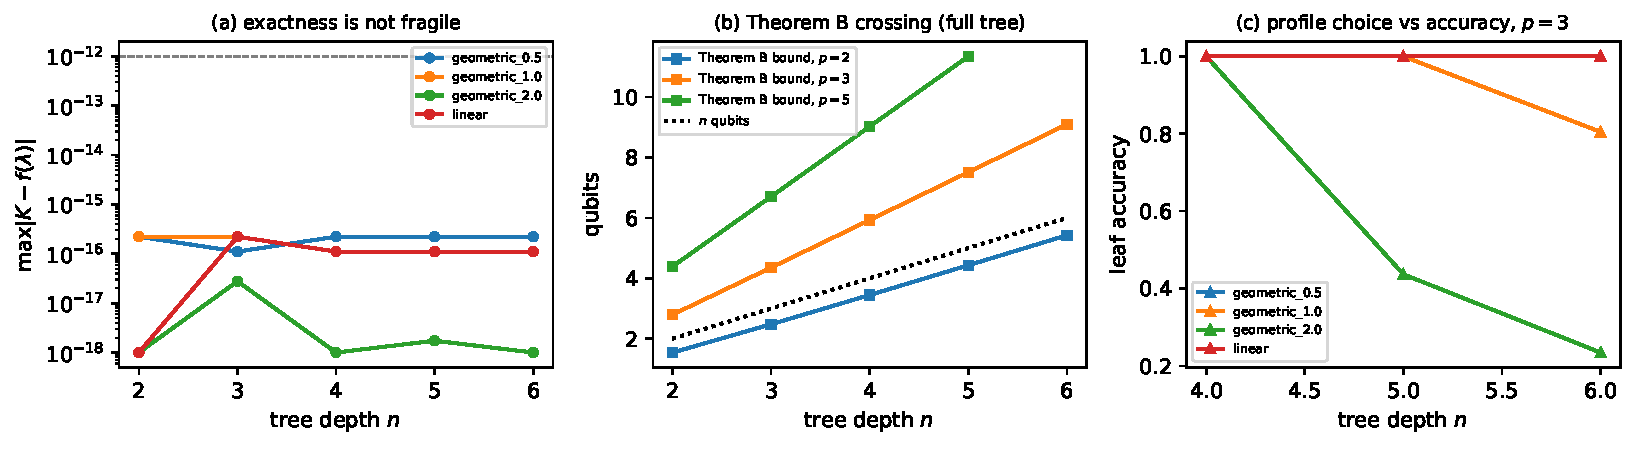
\includegraphics[width=\linewidth]{figures/e3_ablation}
  \caption{E3. (a) The profile residual stays at machine precision for every strictly
    monotone profile at every depth. (b) The \Cref{thm:dimension-bound} bound against
    the $n$ qubits a product or IQP encoding provides: above the diagonal for
    $p \ge 3$, below it for $p = 2$. (c) Profile choice against accuracy.}
  \label{fig:e3-ablation}
\end{figure}

Panel~(a) is the robustness check for \Cref{thm:path-states}: the worst residual over
all $\EThreeConfigs$ configurations is $\EThreeWorstResidual$, and the total number of
strong-triangle violations is $\EThreeMaxViolations$. Exactness does not degrade with
depth, radix or profile shape.

Panel~(b) is the picture of \Cref{cor:no-n-qubit}. For $p = 3$ and $p = 5$ the required
qubit count runs above the diagonal at every depth, so no $n$-qubit encoding can
realise the kernel. For $p = 2$ it runs below, which is \Cref{rem:complementarity}: at
radix two the dimension bound alone is not enough and \Cref{thm:product-nogo} carries
the argument. The curves use the closed form \cref{eq:row-sum} on the full tree, since
an estimate from a subsample saturates at $\log_2$ of the sample size.

\subsection{E4: the re-uploading trade-off}
\label{subsec:e4}

\begin{figure}
  \centering
  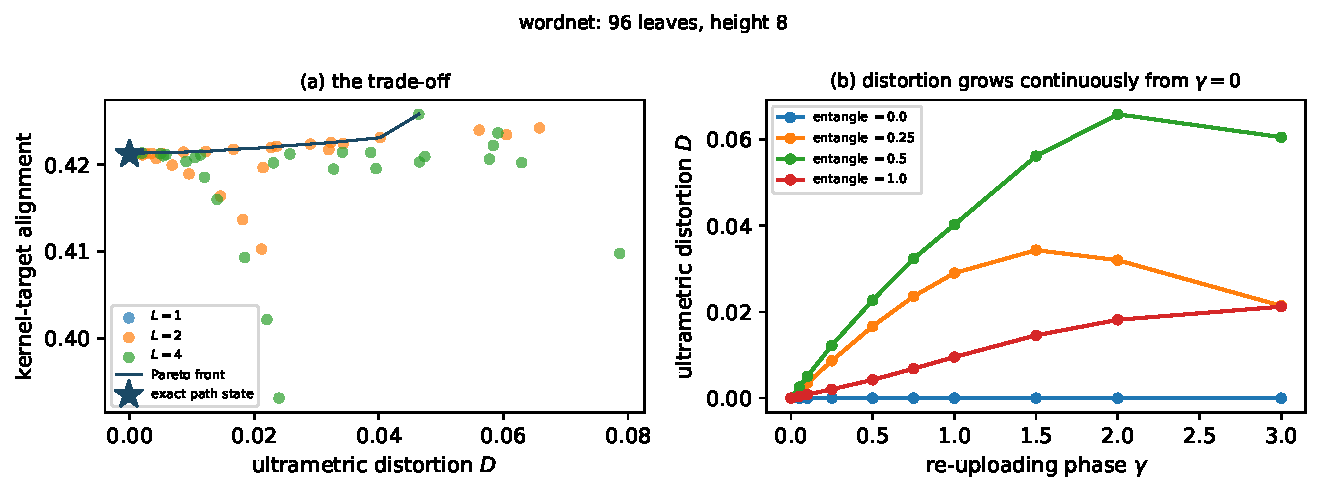
\includegraphics[width=\linewidth]{figures/e4_pareto}
  \caption{E4 on WordNet, over $\EFourConfigs$ configurations of the family
    \cref{eq:reupload}. Distortion grows continuously from zero, so the exact
    construction is the endpoint of a tunable family rather than an isolated point ---
    but the alignment available in exchange is small.}
  \label{fig:e4-pareto}
\end{figure}

Distortion grows continuously from zero as the re-uploading phase increases, which
answers the structural question: the exact construction is not an isolated special
case but the zero-distortion endpoint of a continuum. The quantitative answer is less
encouraging. The exact point achieves alignment $\EFourExactAlignment$, and the best
configuration anywhere in the family achieves $\EFourBestAlignment$ at distortion
$\EFourBestDistortion$, a gain of $\EFourAlignmentGain$. On these datasets the
trade-off exists but buys very little, and we would not recommend paying for it.

\subsection{E5: noise and finite shots}
\label{subsec:e5}

\begin{figure}
  \centering
  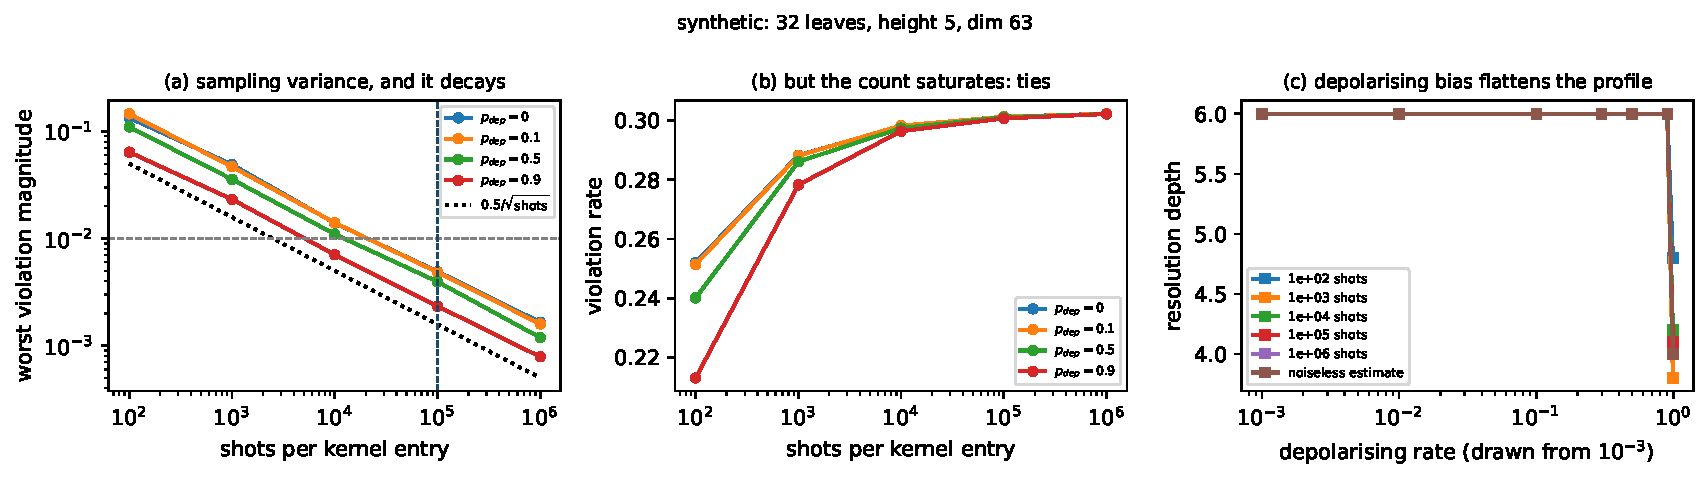
\includegraphics[width=\linewidth]{figures/e5_noise}
  \caption{E5. (a) The violation magnitude decays as $O(1/\sqrt{\text{shots}})$,
    tracking the dotted reference line. (b) The violation \emph{count} saturates
    instead, because a constant fraction of triples in an ultrametric is exactly tight.
    (c) Depolarising noise leaves ultrametricity intact but flattens the profile until
    resolution collapses.}
  \label{fig:e5-noise}
\end{figure}

\Cref{prop:depolarising} predicts that depolarising noise cannot break ultrametricity,
and the measurement agrees exactly: at every rate up to $0.99$, the noiseless-estimate
row has zero violations and zero excess. What degrades is resolution, and only at
extreme rates.

Finite sampling is the real constraint, and measuring it correctly required abandoning
the obvious statistic. The violation count \emph{increases} with the shot budget,
rising towards a plateau, which looks like a bug and is not: $\TieFraction$ of triples
in this ultrametric meet \cref{eq:strong-triangle} with equality, and any perturbation
flips about half of them, so the count converges to that tie fraction rather than to
zero. The violation magnitude behaves as expected, falling from $\ExcessAtLowShots$ at
$\ExcessAtLowShotsCount$ shots to $\ExcessAtHighShots$ at $\ExcessAtHighShotsCount$
shots, a factor of $\sqrt{10}$ per decade. Defining the budget on the magnitude gives
\textbf{$\ShotBudget$ shots per kernel entry} for a worst-case excess below
$\ShotTargetExcess$, over $\ENoiseRepeats$ repetitions.

%% 09-related-work
\section{Related Work}
\label{sec:related-work}

\todo{Draft pending.}

%% 10-limitations
\section{Limitations and Outlook}
\label{sec:limitations}

\paragraph{No quantum speedup in kernel evaluation.}
Restating the point of \Cref{sec:introduction} where a reader will look for it:
$K(x,y) = f(\lcadepth(x,y))$ is computable classically in time linear in the tree
depth, so nothing here accelerates kernel evaluation. The obstructions of
\Cref{thm:product-nogo,thm:dimension-bound} constrain quantum encoding design, and the
construction of \Cref{thm:path-states} is useful as an input stage for deeper quantum
models, where the closed form does not survive subsequent layers. Neither is a speedup
claim.

\paragraph{Multiple inheritance is discarded.}
All three real hierarchies are directed acyclic graphs, and the longest-path reduction
of \Cref{subsec:setup} throws away every hypernym but one. A synset with two genuinely
distinct parents is misrepresented. Extending the construction to DAGs is not a matter
of a better reduction: the ancestor sets of two leaves in a DAG need not be nested, and
\cref{eq:overlap} --- the entire content of \Cref{thm:path-states} --- depends on that
nesting.

\paragraph{Truncation.}
Comparing against $2^{\text{height}}$-dimensional baselines forced a depth-$8$
truncation. The path-state encoding itself has no such limit --- \Cref{tab:resources}
gives $17$ qubits for the untruncated WordNet hierarchy --- so the truncation is a
constraint of the comparison, not of the method. We have not measured the baselines at
full depth, because they cannot be represented there.

\paragraph{The dimension bound is loose for flat profiles.}
\Cref{thm:dimension-bound} is strong when the profile decays quickly and weak when it
does not, and \Cref{rem:s-greater-one} shows the hypothesis $s > 1$ is necessary rather
than convenient. For slowly decaying profiles the bound does not rule out narrow
encodings, and we do not know whether narrow encodings actually exist in that regime.

\paragraph{Simulation only.}
Everything here is statevector simulation. \Cref{prop:depolarising} covers the global
depolarising channel analytically, and \Cref{subsec:e5} gives a shot budget of
$\ShotBudget$ per kernel entry, but coherent errors, readout error and device-specific
noise are untested. The shot budget is also per entry, so a full $m \times m$ kernel
matrix costs $O(m^{2})$ times that, which is the practical barrier to using this at
scale on hardware.

\paragraph{E2 is parity evidence, not a win.}
As reported in \Cref{subsec:e2}, the path state loses on classification accuracy to
both a random product map and to v-PuNNs. The paper's claims rest on
\Cref{thm:product-nogo,thm:dimension-bound,thm:path-states} and on E1, not on E2.

\paragraph{Outlook.}
Three directions seem worth pursuing. The most immediate is using the path state as the
input layer of a deeper variational model, where \Cref{subsec:e4} suggests the
interesting regime is small distortion rather than large. The second is the $p$-adic
connection: the encoding lives in the state space of quantum walks on the $p$-adic tree
\citep{ZunigaGalindo2024QuantumWalks}, and relating the profile $f$ to the spectrum of
a walk generator would give a dynamical reading of what is currently a static
construction. The third is gate synthesis by $p$-adic descent, where the ultrametric
structure would organise the search rather than the data; that is a longer project and
we mention it only to place the present work.

%% 11-conclusion
\section{Conclusion}
\label{sec:conclusion}

\todo{Draft pending.}


\section*{Declaration on Generative AI}
\todo{Complete per the CEUR-WS generative-AI disclosure policy in force at submission.}

\bibliographystyle{elsarticle-num-names}
\bibliography{refs}

\end{document}
